\documentclass[twoside]{book}

% Packages required by doxygen
\usepackage{fixltx2e}
\usepackage{calc}
\usepackage{doxygen}
\usepackage[export]{adjustbox} % also loads graphicx
\usepackage{graphicx}
\usepackage[utf8]{inputenc}
\usepackage{makeidx}
\usepackage{multicol}
\usepackage{multirow}
\PassOptionsToPackage{warn}{textcomp}
\usepackage{textcomp}
\usepackage[nointegrals]{wasysym}
\usepackage[table]{xcolor}

% Font selection
\usepackage[T1]{fontenc}
\usepackage[scaled=.90]{helvet}
\usepackage{courier}
\usepackage{amssymb}
\usepackage{sectsty}
\renewcommand{\familydefault}{\sfdefault}
\allsectionsfont{%
  \fontseries{bc}\selectfont%
  \color{darkgray}%
}
\renewcommand{\DoxyLabelFont}{%
  \fontseries{bc}\selectfont%
  \color{darkgray}%
}
\newcommand{\+}{\discretionary{\mbox{\scriptsize$\hookleftarrow$}}{}{}}

% Page & text layout
\usepackage{geometry}
\geometry{%
  a4paper,%
  top=2.5cm,%
  bottom=2.5cm,%
  left=2.5cm,%
  right=2.5cm%
}
\tolerance=750
\hfuzz=15pt
\hbadness=750
\setlength{\emergencystretch}{15pt}
\setlength{\parindent}{0cm}
\setlength{\parskip}{0.2cm}
\makeatletter
\renewcommand{\paragraph}{%
  \@startsection{paragraph}{4}{0ex}{-1.0ex}{1.0ex}{%
    \normalfont\normalsize\bfseries\SS@parafont%
  }%
}
\renewcommand{\subparagraph}{%
  \@startsection{subparagraph}{5}{0ex}{-1.0ex}{1.0ex}{%
    \normalfont\normalsize\bfseries\SS@subparafont%
  }%
}
\makeatother

% Headers & footers
\usepackage{fancyhdr}
\pagestyle{fancyplain}
\fancyhead[LE]{\fancyplain{}{\bfseries\thepage}}
\fancyhead[CE]{\fancyplain{}{}}
\fancyhead[RE]{\fancyplain{}{\bfseries\leftmark}}
\fancyhead[LO]{\fancyplain{}{\bfseries\rightmark}}
\fancyhead[CO]{\fancyplain{}{}}
\fancyhead[RO]{\fancyplain{}{\bfseries\thepage}}
\fancyfoot[LE]{\fancyplain{}{}}
\fancyfoot[CE]{\fancyplain{}{}}
\fancyfoot[RE]{\fancyplain{}{\bfseries\scriptsize Generated on Wed May 25 2016 18\+:10\+:31 for Bebop\+Drone\+Decode\+Stream by Doxygen }}
\fancyfoot[LO]{\fancyplain{}{\bfseries\scriptsize Generated on Wed May 25 2016 18\+:10\+:31 for Bebop\+Drone\+Decode\+Stream by Doxygen }}
\fancyfoot[CO]{\fancyplain{}{}}
\fancyfoot[RO]{\fancyplain{}{}}
\renewcommand{\footrulewidth}{0.4pt}
\renewcommand{\chaptermark}[1]{%
  \markboth{#1}{}%
}
\renewcommand{\sectionmark}[1]{%
  \markright{\thesection\ #1}%
}

% Indices & bibliography
\usepackage{natbib}
\usepackage[titles]{tocloft}
\setcounter{tocdepth}{3}
\setcounter{secnumdepth}{5}
\makeindex

% Hyperlinks (required, but should be loaded last)
\usepackage{ifpdf}
\ifpdf
  \usepackage[pdftex,pagebackref=true]{hyperref}
\else
  \usepackage[ps2pdf,pagebackref=true]{hyperref}
\fi
\hypersetup{%
  colorlinks=true,%
  linkcolor=blue,%
  citecolor=blue,%
  unicode%
}

% Custom commands
\newcommand{\clearemptydoublepage}{%
  \newpage{\pagestyle{empty}\cleardoublepage}%
}


%===== C O N T E N T S =====

\begin{document}

% Titlepage & ToC
\hypersetup{pageanchor=false,
             bookmarks=true,
             bookmarksnumbered=true,
             pdfencoding=unicode
            }
\pagenumbering{roman}
\begin{titlepage}
\vspace*{7cm}
\begin{center}%
{\Large Bebop\+Drone\+Decode\+Stream }\\
\vspace*{1cm}
{\large Generated by Doxygen 1.8.9.1}\\
\vspace*{0.5cm}
{\small Wed May 25 2016 18:10:31}\\
\end{center}
\end{titlepage}
\clearemptydoublepage
\tableofcontents
\clearemptydoublepage
\pagenumbering{arabic}
\hypersetup{pageanchor=true}

%--- Begin generated contents ---
\chapter{Purpose of Bebop\+Drone\+Decode\+Stream}
\label{md_README}
\hypertarget{md_README}{}
This sample shows how to receive video stream from a Bebop Drone, decode it, display the decoded stream with mplayer and get inputs from users to control the Bebop drone.

\section*{To compile S\+D\+K Example Bebop\+Drone\+Decode\+Stream }

On Linux and Mac\+O\+S X platform \+: make

\section*{Dependencies of Bebop\+Drone\+Decode\+Stream }

You will need {\bfseries mplayer} to show the video stream, {\bfseries ffmpeg} to get the video decoded and {\bfseries ncurse} to get inputs from console

On Linux you can get ncurses-\/dev apt-\/get\+: apt-\/get install ncurses-\/dev

\section*{To run S\+D\+K Example Bebop\+Drone\+Decode\+Stream }

On Linux and Mac\+O\+S X platform \+: make run

\section*{To clean the compilation of Bebop\+Drone\+Decode\+Stream }

On Linux and Mac\+O\+S X platform \+: make clean

\section*{Discussion about Bebop\+Drone\+Decode\+Stream }

This project is separated into 3 classes \+:


\begin{DoxyItemize}
\item Bebop\+Drone\+Decode\+Stream \+: This is the main class. It will operate the connexion to the drone, the setup of the network and video part. It will also register for commands callback and send commands. If you need to add callbacks, add it in register\+A\+R\+Commands\+Callbacks.
\end{DoxyItemize}

In this class, the callback for a new frame received will be called. When it does, it will take a free empty frame from a pool (to avoid an allocation each time a frame is received), put the received data in this free frame and add the free frame to a frame buffer. An other thread will loop, and try to take a frame and pass it to the decoder. Once the frame has been decoded, it will write the decoded frame in a pipe file. M\+Player will read this pipe file and display the frames.


\begin{DoxyItemize}
\item Decoder\+Manager This is an util class that will perform h264 frame decoding thanks to ffmpeg.
\item ihm This is an util class that will catch inputs from console and send these events to Bebop\+Drone\+Decode\+Stream. It will also display some pieces of information about the drone, like its battery level and its flying state.
\end{DoxyItemize}

When you run this sample, be sure to be in the console to catch your keyboard event. As M\+Player will open a new window, you could have to click again in the console. The ihm inputs are implemented on an azerty keyboard. Feel free to adapt it just by changing the key comparison in the function I\+H\+M\+\_\+\+Input\+Processing. 
\chapter{Class Index}
\section{Class List}
Here are the classes, structs, unions and interfaces with brief descriptions\+:\begin{DoxyCompactList}
\item\contentsline{section}{\hyperlink{structIHM__t}{I\+H\+M\+\_\+t} }{\pageref{structIHM__t}}{}
\end{DoxyCompactList}

\chapter{File Index}
\section{File List}
Here is a list of all documented files with brief descriptions\+:\begin{DoxyCompactList}
\item\contentsline{section}{\hyperlink{BebopPiloting_8c}{Bebop\+Piloting.\+c} \\*This file contains sources about basic arsdk example sending commands to a bebop drone for piloting it and make it jump it and receiving its battery level }{\pageref{BebopPiloting_8c}}{}
\item\contentsline{section}{{\bfseries Bebop\+Piloting.\+h} }{\pageref{BebopPiloting_8h}}{}
\item\contentsline{section}{\hyperlink{ihm_8c}{ihm.\+c} \\*This file contains sources about ncurses I\+H\+M used by arsdk example \char`\"{}\+Jumping\+Sumo\+Piloting\char`\"{} }{\pageref{ihm_8c}}{}
\item\contentsline{section}{{\bfseries ihm.\+h} }{\pageref{ihm_8h}}{}
\end{DoxyCompactList}

\chapter{Class Documentation}
\hypertarget{struct__ARCODECS__Manager__Component__t__}{}\section{\+\_\+\+A\+R\+C\+O\+D\+E\+C\+S\+\_\+\+Manager\+\_\+\+Component\+\_\+t\+\_\+ Struct Reference}
\label{struct__ARCODECS__Manager__Component__t__}\index{\+\_\+\+A\+R\+C\+O\+D\+E\+C\+S\+\_\+\+Manager\+\_\+\+Component\+\_\+t\+\_\+@{\+\_\+\+A\+R\+C\+O\+D\+E\+C\+S\+\_\+\+Manager\+\_\+\+Component\+\_\+t\+\_\+}}


Component of a frame.  




{\ttfamily \#include $<$Decoder\+Manager.\+h$>$}

\subsection*{Public Attributes}
\begin{DoxyCompactItemize}
\item 
uint8\+\_\+t $\ast$ \hyperlink{struct__ARCODECS__Manager__Component__t___a606943eddf1c545ab336a2d572a20d0e}{data}
\item 
uint32\+\_\+t \hyperlink{struct__ARCODECS__Manager__Component__t___a69699f5b967723699ccb523484808ab9}{line\+Size}
\item 
uint32\+\_\+t \hyperlink{struct__ARCODECS__Manager__Component__t___a30b2f6ff9dd1fccb7053a092ccb0f107}{size}
\end{DoxyCompactItemize}


\subsection{Detailed Description}
Component of a frame. 

\subsection{Member Data Documentation}
\hypertarget{struct__ARCODECS__Manager__Component__t___a606943eddf1c545ab336a2d572a20d0e}{}\index{\+\_\+\+A\+R\+C\+O\+D\+E\+C\+S\+\_\+\+Manager\+\_\+\+Component\+\_\+t\+\_\+@{\+\_\+\+A\+R\+C\+O\+D\+E\+C\+S\+\_\+\+Manager\+\_\+\+Component\+\_\+t\+\_\+}!data@{data}}
\index{data@{data}!\+\_\+\+A\+R\+C\+O\+D\+E\+C\+S\+\_\+\+Manager\+\_\+\+Component\+\_\+t\+\_\+@{\+\_\+\+A\+R\+C\+O\+D\+E\+C\+S\+\_\+\+Manager\+\_\+\+Component\+\_\+t\+\_\+}}
\subsubsection[{data}]{\setlength{\rightskip}{0pt plus 5cm}uint8\+\_\+t$\ast$ \+\_\+\+A\+R\+C\+O\+D\+E\+C\+S\+\_\+\+Manager\+\_\+\+Component\+\_\+t\+\_\+\+::data}\label{struct__ARCODECS__Manager__Component__t___a606943eddf1c545ab336a2d572a20d0e}
data buffer \hypertarget{struct__ARCODECS__Manager__Component__t___a69699f5b967723699ccb523484808ab9}{}\index{\+\_\+\+A\+R\+C\+O\+D\+E\+C\+S\+\_\+\+Manager\+\_\+\+Component\+\_\+t\+\_\+@{\+\_\+\+A\+R\+C\+O\+D\+E\+C\+S\+\_\+\+Manager\+\_\+\+Component\+\_\+t\+\_\+}!line\+Size@{line\+Size}}
\index{line\+Size@{line\+Size}!\+\_\+\+A\+R\+C\+O\+D\+E\+C\+S\+\_\+\+Manager\+\_\+\+Component\+\_\+t\+\_\+@{\+\_\+\+A\+R\+C\+O\+D\+E\+C\+S\+\_\+\+Manager\+\_\+\+Component\+\_\+t\+\_\+}}
\subsubsection[{line\+Size}]{\setlength{\rightskip}{0pt plus 5cm}uint32\+\_\+t \+\_\+\+A\+R\+C\+O\+D\+E\+C\+S\+\_\+\+Manager\+\_\+\+Component\+\_\+t\+\_\+\+::line\+Size}\label{struct__ARCODECS__Manager__Component__t___a69699f5b967723699ccb523484808ab9}
size of each line of the component \hypertarget{struct__ARCODECS__Manager__Component__t___a30b2f6ff9dd1fccb7053a092ccb0f107}{}\index{\+\_\+\+A\+R\+C\+O\+D\+E\+C\+S\+\_\+\+Manager\+\_\+\+Component\+\_\+t\+\_\+@{\+\_\+\+A\+R\+C\+O\+D\+E\+C\+S\+\_\+\+Manager\+\_\+\+Component\+\_\+t\+\_\+}!size@{size}}
\index{size@{size}!\+\_\+\+A\+R\+C\+O\+D\+E\+C\+S\+\_\+\+Manager\+\_\+\+Component\+\_\+t\+\_\+@{\+\_\+\+A\+R\+C\+O\+D\+E\+C\+S\+\_\+\+Manager\+\_\+\+Component\+\_\+t\+\_\+}}
\subsubsection[{size}]{\setlength{\rightskip}{0pt plus 5cm}uint32\+\_\+t \+\_\+\+A\+R\+C\+O\+D\+E\+C\+S\+\_\+\+Manager\+\_\+\+Component\+\_\+t\+\_\+\+::size}\label{struct__ARCODECS__Manager__Component__t___a30b2f6ff9dd1fccb7053a092ccb0f107}
size of the buffer 

The documentation for this struct was generated from the following file\+:\begin{DoxyCompactItemize}
\item 
Decoder\+Manager.\+h\end{DoxyCompactItemize}

\hypertarget{struct__ARCODECS__Manager__FFMPEGDecoder__t__}{}\section{\+\_\+\+A\+R\+C\+O\+D\+E\+C\+S\+\_\+\+Manager\+\_\+\+F\+F\+M\+P\+E\+G\+Decoder\+\_\+t\+\_\+ Struct Reference}
\label{struct__ARCODECS__Manager__FFMPEGDecoder__t__}\index{\+\_\+\+A\+R\+C\+O\+D\+E\+C\+S\+\_\+\+Manager\+\_\+\+F\+F\+M\+P\+E\+G\+Decoder\+\_\+t\+\_\+@{\+\_\+\+A\+R\+C\+O\+D\+E\+C\+S\+\_\+\+Manager\+\_\+\+F\+F\+M\+P\+E\+G\+Decoder\+\_\+t\+\_\+}}
\subsection*{Public Attributes}
\begin{DoxyCompactItemize}
\item 
\hypertarget{struct__ARCODECS__Manager__FFMPEGDecoder__t___a54f960af3b215ad993feedca5dda5c2d}{}A\+V\+Codec $\ast$ {\bfseries codec}\label{struct__ARCODECS__Manager__FFMPEGDecoder__t___a54f960af3b215ad993feedca5dda5c2d}

\item 
\hypertarget{struct__ARCODECS__Manager__FFMPEGDecoder__t___ab35630e0b6d4d961106a3b031047ff1e}{}A\+V\+Codec\+Context $\ast$ {\bfseries codec\+Ctx}\label{struct__ARCODECS__Manager__FFMPEGDecoder__t___ab35630e0b6d4d961106a3b031047ff1e}

\item 
\hypertarget{struct__ARCODECS__Manager__FFMPEGDecoder__t___a13410d1f5c4992e7c9b507a632e4ef9e}{}A\+V\+Frame $\ast$ {\bfseries decoded\+Frame}\label{struct__ARCODECS__Manager__FFMPEGDecoder__t___a13410d1f5c4992e7c9b507a632e4ef9e}

\item 
\hypertarget{struct__ARCODECS__Manager__FFMPEGDecoder__t___ac84534612a21669b931a651698dbba1d}{}A\+V\+Packet {\bfseries avpkt}\label{struct__ARCODECS__Manager__FFMPEGDecoder__t___ac84534612a21669b931a651698dbba1d}

\item 
\hypertarget{struct__ARCODECS__Manager__FFMPEGDecoder__t___a44bd4d2dd5436480d25c27fd013c0b3d}{}uint8\+\_\+t $\ast$ {\bfseries output\+Data}\label{struct__ARCODECS__Manager__FFMPEGDecoder__t___a44bd4d2dd5436480d25c27fd013c0b3d}

\item 
\hypertarget{struct__ARCODECS__Manager__FFMPEGDecoder__t___a298ee2088fdb2f7798bce2c99bec22e0}{}int {\bfseries output\+Data\+Size}\label{struct__ARCODECS__Manager__FFMPEGDecoder__t___a298ee2088fdb2f7798bce2c99bec22e0}

\end{DoxyCompactItemize}


The documentation for this struct was generated from the following file\+:\begin{DoxyCompactItemize}
\item 
Decoder\+Manager.\+c\end{DoxyCompactItemize}

\hypertarget{struct__ARCODECS__Manager__Frame__t__}{}\section{\+\_\+\+A\+R\+C\+O\+D\+E\+C\+S\+\_\+\+Manager\+\_\+\+Frame\+\_\+t\+\_\+ Struct Reference}
\label{struct__ARCODECS__Manager__Frame__t__}\index{\+\_\+\+A\+R\+C\+O\+D\+E\+C\+S\+\_\+\+Manager\+\_\+\+Frame\+\_\+t\+\_\+@{\+\_\+\+A\+R\+C\+O\+D\+E\+C\+S\+\_\+\+Manager\+\_\+\+Frame\+\_\+t\+\_\+}}


Video and audio codecs manager allow to decode video and audio.  




{\ttfamily \#include $<$Decoder\+Manager.\+h$>$}



Collaboration diagram for \+\_\+\+A\+R\+C\+O\+D\+E\+C\+S\+\_\+\+Manager\+\_\+\+Frame\+\_\+t\+\_\+\+:
\nopagebreak
\begin{figure}[H]
\begin{center}
\leavevmode
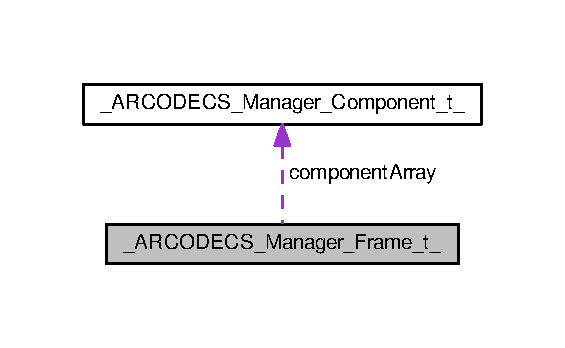
\includegraphics[width=271pt]{struct__ARCODECS__Manager__Frame__t____coll__graph}
\end{center}
\end{figure}
\subsection*{Public Attributes}
\begin{DoxyCompactItemize}
\item 
\hypertarget{struct__ARCODECS__Manager__Frame__t___a4d166b423ec535a87c6b8af430962eae}{}e\+A\+R\+C\+O\+D\+E\+C\+S\+\_\+\+F\+O\+R\+M\+A\+T {\bfseries format}\label{struct__ARCODECS__Manager__Frame__t___a4d166b423ec535a87c6b8af430962eae}

\item 
\hypertarget{struct__ARCODECS__Manager__Frame__t___a7429d7be2c65a64558b087e076250b08}{}uint32\+\_\+t {\bfseries width}\label{struct__ARCODECS__Manager__Frame__t___a7429d7be2c65a64558b087e076250b08}

\item 
\hypertarget{struct__ARCODECS__Manager__Frame__t___a553fa419c0a93a12e67a3f24ffa9a3bf}{}uint32\+\_\+t {\bfseries height}\label{struct__ARCODECS__Manager__Frame__t___a553fa419c0a93a12e67a3f24ffa9a3bf}

\item 
\hypertarget{struct__ARCODECS__Manager__Frame__t___a599595f4fceb2f0ca330c14780da468f}{}uint32\+\_\+t {\bfseries number\+Of\+Component}\label{struct__ARCODECS__Manager__Frame__t___a599595f4fceb2f0ca330c14780da468f}

\item 
\hypertarget{struct__ARCODECS__Manager__Frame__t___afee2d4971c9a9dcaeb9fc2b1d182727c}{}\hyperlink{struct__ARCODECS__Manager__Component__t__}{A\+R\+C\+O\+D\+E\+C\+S\+\_\+\+Manager\+\_\+\+Component\+\_\+t} $\ast$ {\bfseries component\+Array}\label{struct__ARCODECS__Manager__Frame__t___afee2d4971c9a9dcaeb9fc2b1d182727c}

\end{DoxyCompactItemize}


\subsection{Detailed Description}
Video and audio codecs manager allow to decode video and audio. 

The documentation for this struct was generated from the following file\+:\begin{DoxyCompactItemize}
\item 
Decoder\+Manager.\+h\end{DoxyCompactItemize}

\hypertarget{struct__ARDrone3CameraData__t__}{}\section{\+\_\+\+A\+R\+Drone3\+Camera\+Data\+\_\+t\+\_\+ Struct Reference}
\label{struct__ARDrone3CameraData__t__}\index{\+\_\+\+A\+R\+Drone3\+Camera\+Data\+\_\+t\+\_\+@{\+\_\+\+A\+R\+Drone3\+Camera\+Data\+\_\+t\+\_\+}}
\subsection*{Public Attributes}
\begin{DoxyCompactItemize}
\item 
\hypertarget{struct__ARDrone3CameraData__t___ad7502c8c0a61a2631c2047701f2a0ca0}{}int {\bfseries tilt}\label{struct__ARDrone3CameraData__t___ad7502c8c0a61a2631c2047701f2a0ca0}

\item 
\hypertarget{struct__ARDrone3CameraData__t___ac11aa79599aeef7ca412d83fc23672a3}{}int {\bfseries pan}\label{struct__ARDrone3CameraData__t___ac11aa79599aeef7ca412d83fc23672a3}

\end{DoxyCompactItemize}


The documentation for this struct was generated from the following file\+:\begin{DoxyCompactItemize}
\item 
Bebop\+Drone\+Decode\+Stream.\+h\end{DoxyCompactItemize}

\hypertarget{structARCODECS__Manager__t}{}\section{A\+R\+C\+O\+D\+E\+C\+S\+\_\+\+Manager\+\_\+t Struct Reference}
\label{structARCODECS__Manager__t}\index{A\+R\+C\+O\+D\+E\+C\+S\+\_\+\+Manager\+\_\+t@{A\+R\+C\+O\+D\+E\+C\+S\+\_\+\+Manager\+\_\+t}}


Video and audio codecs manager structure allow to decode video and audio.  




Collaboration diagram for A\+R\+C\+O\+D\+E\+C\+S\+\_\+\+Manager\+\_\+t\+:
\nopagebreak
\begin{figure}[H]
\begin{center}
\leavevmode
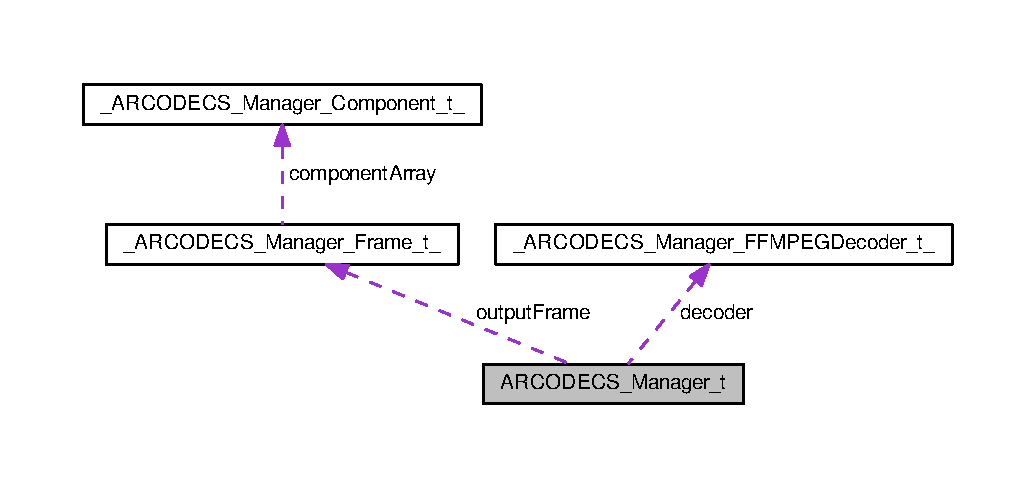
\includegraphics[width=350pt]{structARCODECS__Manager__t__coll__graph}
\end{center}
\end{figure}
\subsection*{Public Attributes}
\begin{DoxyCompactItemize}
\item 
\hypertarget{structARCODECS__Manager__t_a2dce3f7515b7473133d402162399bfa8}{}A\+R\+C\+O\+D\+E\+C\+S\+\_\+\+Manager\+\_\+\+Get\+Next\+Data\+Callback\+\_\+t {\bfseries callback}\label{structARCODECS__Manager__t_a2dce3f7515b7473133d402162399bfa8}

\item 
\hypertarget{structARCODECS__Manager__t_aaccf39b085a379cd2493a3731c6c3c3a}{}void $\ast$ {\bfseries callback\+Custom\+Data}\label{structARCODECS__Manager__t_aaccf39b085a379cd2493a3731c6c3c3a}

\item 
\hypertarget{structARCODECS__Manager__t_a7246195626a8fac847a5d836c8942c4b}{}\hyperlink{struct__ARCODECS__Manager__FFMPEGDecoder__t__}{A\+R\+C\+O\+D\+E\+C\+S\+\_\+\+Manager\+\_\+\+F\+F\+M\+P\+E\+G\+Decoder\+\_\+t} $\ast$ {\bfseries decoder}\label{structARCODECS__Manager__t_a7246195626a8fac847a5d836c8942c4b}

\item 
\hypertarget{structARCODECS__Manager__t_a318ac83874092f41424a5e6a7774dc50}{}\hyperlink{struct__ARCODECS__Manager__Frame__t__}{A\+R\+C\+O\+D\+E\+C\+S\+\_\+\+Manager\+\_\+\+Frame\+\_\+t} {\bfseries output\+Frame}\label{structARCODECS__Manager__t_a318ac83874092f41424a5e6a7774dc50}

\end{DoxyCompactItemize}


\subsection{Detailed Description}
Video and audio codecs manager structure allow to decode video and audio. 

The documentation for this struct was generated from the following file\+:\begin{DoxyCompactItemize}
\item 
Decoder\+Manager.\+c\end{DoxyCompactItemize}

\hypertarget{structBD__MANAGER__t}{}\section{B\+D\+\_\+\+M\+A\+N\+A\+G\+E\+R\+\_\+t Struct Reference}
\label{structBD__MANAGER__t}\index{B\+D\+\_\+\+M\+A\+N\+A\+G\+E\+R\+\_\+t@{B\+D\+\_\+\+M\+A\+N\+A\+G\+E\+R\+\_\+t}}


Collaboration diagram for B\+D\+\_\+\+M\+A\+N\+A\+G\+E\+R\+\_\+t\+:
\nopagebreak
\begin{figure}[H]
\begin{center}
\leavevmode
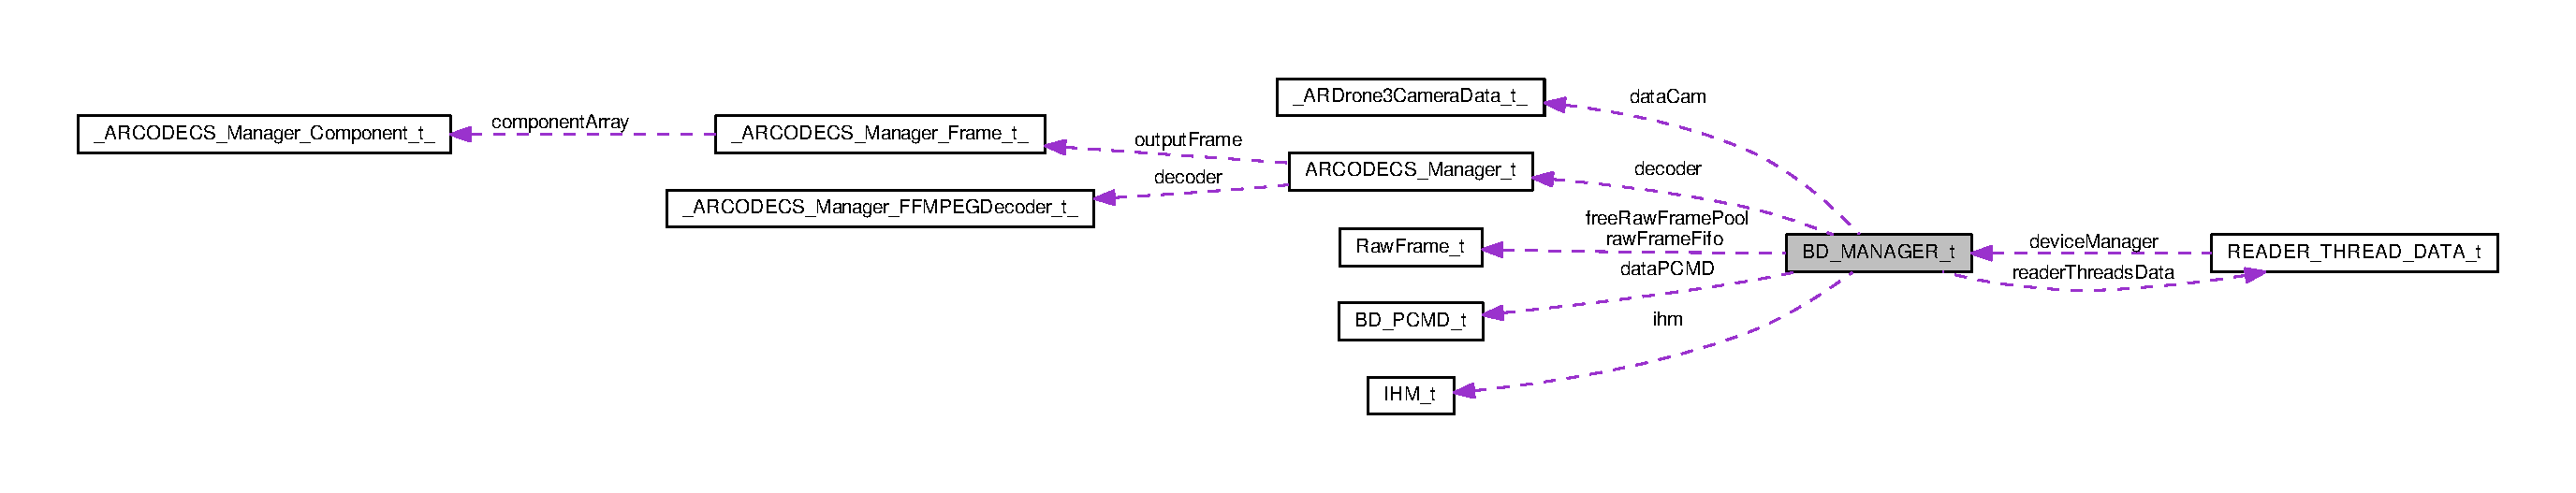
\includegraphics[width=350pt]{structBD__MANAGER__t__coll__graph}
\end{center}
\end{figure}
\subsection*{Public Attributes}
\begin{DoxyCompactItemize}
\item 
\hypertarget{structBD__MANAGER__t_a72f94bb1cd0f3fc17091f33ef86b9854}{}A\+R\+N\+E\+T\+W\+O\+R\+K\+A\+L\+\_\+\+Manager\+\_\+t $\ast$ {\bfseries al\+Manager}\label{structBD__MANAGER__t_a72f94bb1cd0f3fc17091f33ef86b9854}

\item 
\hypertarget{structBD__MANAGER__t_aa206d61e05f8bbd07c8f2fb95fb2c9de}{}A\+R\+N\+E\+T\+W\+O\+R\+K\+\_\+\+Manager\+\_\+t $\ast$ {\bfseries net\+Manager}\label{structBD__MANAGER__t_aa206d61e05f8bbd07c8f2fb95fb2c9de}

\item 
\hypertarget{structBD__MANAGER__t_aa4299944778f151a55ee726fe1ac1c5b}{}A\+R\+S\+T\+R\+E\+A\+M\+\_\+\+Reader\+\_\+t $\ast$ {\bfseries stream\+Reader}\label{structBD__MANAGER__t_aa4299944778f151a55ee726fe1ac1c5b}

\item 
\hypertarget{structBD__MANAGER__t_a09aba83d294e3ca0263e8de3946c76e0}{}A\+R\+S\+A\+L\+\_\+\+Thread\+\_\+t {\bfseries looper\+Thread}\label{structBD__MANAGER__t_a09aba83d294e3ca0263e8de3946c76e0}

\item 
\hypertarget{structBD__MANAGER__t_aa4735b3bb6c989bfcd6cb51e90789b44}{}A\+R\+S\+A\+L\+\_\+\+Thread\+\_\+t {\bfseries rx\+Thread}\label{structBD__MANAGER__t_aa4735b3bb6c989bfcd6cb51e90789b44}

\item 
\hypertarget{structBD__MANAGER__t_a5ab27da27e34c5e76dbbc033fe99d080}{}A\+R\+S\+A\+L\+\_\+\+Thread\+\_\+t {\bfseries tx\+Thread}\label{structBD__MANAGER__t_a5ab27da27e34c5e76dbbc033fe99d080}

\item 
\hypertarget{structBD__MANAGER__t_a14246d06a707dcb4bcf0dc2f541ee09c}{}A\+R\+S\+A\+L\+\_\+\+Thread\+\_\+t {\bfseries video\+Tx\+Thread}\label{structBD__MANAGER__t_a14246d06a707dcb4bcf0dc2f541ee09c}

\item 
\hypertarget{structBD__MANAGER__t_a7b58d261b275c75e79b7345476983e1c}{}A\+R\+S\+A\+L\+\_\+\+Thread\+\_\+t {\bfseries video\+Rx\+Thread}\label{structBD__MANAGER__t_a7b58d261b275c75e79b7345476983e1c}

\item 
\hypertarget{structBD__MANAGER__t_a9bcabdb60dcfffe872d576b2257583fe}{}int {\bfseries d2c\+Port}\label{structBD__MANAGER__t_a9bcabdb60dcfffe872d576b2257583fe}

\item 
\hypertarget{structBD__MANAGER__t_a5dd5fc716f1c7c84031e7e016a0f14f3}{}int {\bfseries c2d\+Port}\label{structBD__MANAGER__t_a5dd5fc716f1c7c84031e7e016a0f14f3}

\item 
\hypertarget{structBD__MANAGER__t_a13d8ac846cffaef4278ee721d2533ea2}{}int {\bfseries arstream\+Frag\+Size}\label{structBD__MANAGER__t_a13d8ac846cffaef4278ee721d2533ea2}

\item 
\hypertarget{structBD__MANAGER__t_a5960ea0c7fb6a963503208d359351c35}{}int {\bfseries arstream\+Frag\+Nb}\label{structBD__MANAGER__t_a5960ea0c7fb6a963503208d359351c35}

\item 
\hypertarget{structBD__MANAGER__t_af1f5ce80cd4b602990108c07d7bc8878}{}int {\bfseries arstream\+Ack\+Delay}\label{structBD__MANAGER__t_af1f5ce80cd4b602990108c07d7bc8878}

\item 
\hypertarget{structBD__MANAGER__t_a525cf5746b18a94ee39b7c38d2eee852}{}uint8\+\_\+t $\ast$ {\bfseries video\+Frame}\label{structBD__MANAGER__t_a525cf5746b18a94ee39b7c38d2eee852}

\item 
\hypertarget{structBD__MANAGER__t_ac9a70352549d704065f93572ff02c774}{}uint32\+\_\+t {\bfseries video\+Frame\+Size}\label{structBD__MANAGER__t_ac9a70352549d704065f93572ff02c774}

\item 
\hypertarget{structBD__MANAGER__t_a139ca18276ef45023fd58f4178df2e7f}{}\hyperlink{structBD__PCMD__t}{B\+D\+\_\+\+P\+C\+M\+D\+\_\+t} {\bfseries data\+P\+C\+M\+D}\label{structBD__MANAGER__t_a139ca18276ef45023fd58f4178df2e7f}

\item 
\hypertarget{structBD__MANAGER__t_a60e12166587af64f82b406cf3906ef95}{}\hyperlink{struct__ARDrone3CameraData__t__}{B\+D\+\_\+\+Cam\+\_\+t} {\bfseries data\+Cam}\label{structBD__MANAGER__t_a60e12166587af64f82b406cf3906ef95}

\item 
\hypertarget{structBD__MANAGER__t_a0b82ea608507316aaecd827dcefac04b}{}\hyperlink{structARCODECS__Manager__t}{A\+R\+C\+O\+D\+E\+C\+S\+\_\+\+Manager\+\_\+t} $\ast$ {\bfseries decoder}\label{structBD__MANAGER__t_a0b82ea608507316aaecd827dcefac04b}

\item 
\hypertarget{structBD__MANAGER__t_a11600d320c86ef6f44c9bc550a366de4}{}int {\bfseries decoding\+Canceled}\label{structBD__MANAGER__t_a11600d320c86ef6f44c9bc550a366de4}

\item 
\hypertarget{structBD__MANAGER__t_a3c9a5b9341aa85c22b72c24f770efbfc}{}A\+R\+S\+A\+L\+\_\+\+Thread\+\_\+t {\bfseries decoding\+Thread}\label{structBD__MANAGER__t_a3c9a5b9341aa85c22b72c24f770efbfc}

\item 
\hypertarget{structBD__MANAGER__t_a54f024337acceb7ce1089601a87ad26a}{}int {\bfseries has\+Received\+First\+I\+Frame}\label{structBD__MANAGER__t_a54f024337acceb7ce1089601a87ad26a}

\item 
\hypertarget{structBD__MANAGER__t_afe2c94ee00d4d7df1bc71c76a2f1d872}{}\hyperlink{structRawFrame__t}{Raw\+Frame\+\_\+t} $\ast$$\ast$ {\bfseries free\+Raw\+Frame\+Pool}\label{structBD__MANAGER__t_afe2c94ee00d4d7df1bc71c76a2f1d872}

\item 
\hypertarget{structBD__MANAGER__t_a84e33c551070a412584db86affa5556e}{}int {\bfseries raw\+Frame\+Pool\+Capacity}\label{structBD__MANAGER__t_a84e33c551070a412584db86affa5556e}

\item 
\hypertarget{structBD__MANAGER__t_acb813713bc178fb42cc105f7286be18d}{}int {\bfseries last\+Raw\+Frame\+Free\+Idx}\label{structBD__MANAGER__t_acb813713bc178fb42cc105f7286be18d}

\item 
\hypertarget{structBD__MANAGER__t_a59e57c4b1aaf89bdbb7cf27f0d648e3b}{}\hyperlink{structRawFrame__t}{Raw\+Frame\+\_\+t} $\ast$$\ast$ {\bfseries raw\+Frame\+Fifo}\label{structBD__MANAGER__t_a59e57c4b1aaf89bdbb7cf27f0d648e3b}

\item 
\hypertarget{structBD__MANAGER__t_ad2248d39ae81fb5b81e10f9973d86ed2}{}int {\bfseries fifo\+Read\+Idx}\label{structBD__MANAGER__t_ad2248d39ae81fb5b81e10f9973d86ed2}

\item 
\hypertarget{structBD__MANAGER__t_a547f77e4bd8b7d19ecbac517f1187cb6}{}int {\bfseries fifo\+Write\+Idx}\label{structBD__MANAGER__t_a547f77e4bd8b7d19ecbac517f1187cb6}

\item 
\hypertarget{structBD__MANAGER__t_a990ba28467879eab9f74dc1abb701e86}{}e\+A\+R\+C\+O\+M\+M\+A\+N\+D\+S\+\_\+\+A\+R\+D\+R\+O\+N\+E3\+\_\+\+P\+I\+L\+O\+T\+I\+N\+G\+S\+T\+A\+T\+E\+\_\+\+F\+L\+Y\+I\+N\+G\+S\+T\+A\+T\+E\+C\+H\+A\+N\+G\+E\+D\+\_\+\+S\+T\+A\+T\+E {\bfseries flying\+State}\label{structBD__MANAGER__t_a990ba28467879eab9f74dc1abb701e86}

\item 
\hypertarget{structBD__MANAGER__t_a6ef2f0ab25b4ec27a0db6e5b2d45f665}{}F\+I\+L\+E $\ast$ {\bfseries video\+\_\+out}\label{structBD__MANAGER__t_a6ef2f0ab25b4ec27a0db6e5b2d45f665}

\item 
\hypertarget{structBD__MANAGER__t_a6e94ed60b9a8b7bf5172f3454179f23a}{}A\+R\+S\+A\+L\+\_\+\+Mutex\+\_\+t {\bfseries mutex}\label{structBD__MANAGER__t_a6e94ed60b9a8b7bf5172f3454179f23a}

\item 
\hypertarget{structBD__MANAGER__t_aa3b7db68f7f44df515ef261d3875fb70}{}A\+R\+S\+A\+L\+\_\+\+Thread\+\_\+t $\ast$ {\bfseries reader\+Threads}\label{structBD__MANAGER__t_aa3b7db68f7f44df515ef261d3875fb70}

\item 
\hypertarget{structBD__MANAGER__t_a8e51ed4fdf0e0bd52030fef9b6c44da2}{}\hyperlink{structREADER__THREAD__DATA__t}{R\+E\+A\+D\+E\+R\+\_\+\+T\+H\+R\+E\+A\+D\+\_\+\+D\+A\+T\+A\+\_\+t} $\ast$ {\bfseries reader\+Threads\+Data}\label{structBD__MANAGER__t_a8e51ed4fdf0e0bd52030fef9b6c44da2}

\item 
\hypertarget{structBD__MANAGER__t_a8a4ceedf2f1c86686f2144e797ec1152}{}int {\bfseries run}\label{structBD__MANAGER__t_a8a4ceedf2f1c86686f2144e797ec1152}

\item 
\hypertarget{structBD__MANAGER__t_a8e71767d59e5387c094236b521cf677c}{}\hyperlink{structIHM__t}{I\+H\+M\+\_\+t} $\ast$ {\bfseries ihm}\label{structBD__MANAGER__t_a8e71767d59e5387c094236b521cf677c}

\end{DoxyCompactItemize}


The documentation for this struct was generated from the following file\+:\begin{DoxyCompactItemize}
\item 
Bebop\+Drone\+Decode\+Stream.\+h\end{DoxyCompactItemize}

\hypertarget{structBD__PCMD__t}{}\section{B\+D\+\_\+\+P\+C\+M\+D\+\_\+t Struct Reference}
\label{structBD__PCMD__t}\index{B\+D\+\_\+\+P\+C\+M\+D\+\_\+t@{B\+D\+\_\+\+P\+C\+M\+D\+\_\+t}}
\subsection*{Public Attributes}
\begin{DoxyCompactItemize}
\item 
\hypertarget{structBD__PCMD__t_ae050fb8b4a35994b40ecc87d718b8586}{}int {\bfseries flag}\label{structBD__PCMD__t_ae050fb8b4a35994b40ecc87d718b8586}

\item 
\hypertarget{structBD__PCMD__t_a15248e2d8fcee22535b19b54a247f8e2}{}int {\bfseries roll}\label{structBD__PCMD__t_a15248e2d8fcee22535b19b54a247f8e2}

\item 
\hypertarget{structBD__PCMD__t_aee46ae9d983395de16707dda985104be}{}int {\bfseries pitch}\label{structBD__PCMD__t_aee46ae9d983395de16707dda985104be}

\item 
\hypertarget{structBD__PCMD__t_aa4ca0a4fcb3ea5c1acfbe31c81679b42}{}int {\bfseries yaw}\label{structBD__PCMD__t_aa4ca0a4fcb3ea5c1acfbe31c81679b42}

\item 
\hypertarget{structBD__PCMD__t_a174a572d645aebfe34e086312f6efdf2}{}int {\bfseries gaz}\label{structBD__PCMD__t_a174a572d645aebfe34e086312f6efdf2}

\end{DoxyCompactItemize}


The documentation for this struct was generated from the following file\+:\begin{DoxyCompactItemize}
\item 
Bebop\+Drone\+Decode\+Stream.\+h\end{DoxyCompactItemize}

\hypertarget{structIHM__t}{}\section{I\+H\+M\+\_\+t Struct Reference}
\label{structIHM__t}\index{I\+H\+M\+\_\+t@{I\+H\+M\+\_\+t}}
\subsection*{Public Attributes}
\begin{DoxyCompactItemize}
\item 
\hypertarget{structIHM__t_a054e97c316934e2c096851218b77eeb0}{}W\+I\+N\+D\+O\+W $\ast$ {\bfseries main\+Window}\label{structIHM__t_a054e97c316934e2c096851218b77eeb0}

\item 
\hypertarget{structIHM__t_a26a01f7024501c6f6cb265a3ec63b51d}{}A\+R\+S\+A\+L\+\_\+\+Thread\+\_\+t {\bfseries input\+Thread}\label{structIHM__t_a26a01f7024501c6f6cb265a3ec63b51d}

\item 
\hypertarget{structIHM__t_a55f137fec8f1a4c6e7f750e867c5f572}{}int {\bfseries run}\label{structIHM__t_a55f137fec8f1a4c6e7f750e867c5f572}

\item 
\hypertarget{structIHM__t_a02dfaefc359fb07336c9489fd8218430}{}I\+H\+M\+\_\+on\+Input\+Event\+\_\+t {\bfseries on\+Input\+Event\+Callback}\label{structIHM__t_a02dfaefc359fb07336c9489fd8218430}

\item 
\hypertarget{structIHM__t_a7c9f6f8a2f01a3418c4690708b8cb910}{}void $\ast$ {\bfseries custom\+Data}\label{structIHM__t_a7c9f6f8a2f01a3418c4690708b8cb910}

\end{DoxyCompactItemize}


The documentation for this struct was generated from the following file\+:\begin{DoxyCompactItemize}
\item 
ihm.\+h\end{DoxyCompactItemize}

\hypertarget{structRawFrame__t}{}\section{Raw\+Frame\+\_\+t Struct Reference}
\label{structRawFrame__t}\index{Raw\+Frame\+\_\+t@{Raw\+Frame\+\_\+t}}


Component of a frame.  


\subsection*{Public Attributes}
\begin{DoxyCompactItemize}
\item 
uint8\+\_\+t $\ast$ \hyperlink{structRawFrame__t_a53d5b44181a7d3160ae6ef910c61df8d}{data}
\item 
uint32\+\_\+t \hyperlink{structRawFrame__t_a3268f9bcece432d3e9bad16cc2c60ece}{size}
\item 
\hypertarget{structRawFrame__t_a8b8217c36048cc707fd04ebd5be39172}{}uint8\+\_\+t {\bfseries is\+Iframe}\label{structRawFrame__t_a8b8217c36048cc707fd04ebd5be39172}

\end{DoxyCompactItemize}


\subsection{Detailed Description}
Component of a frame. 

\subsection{Member Data Documentation}
\hypertarget{structRawFrame__t_a53d5b44181a7d3160ae6ef910c61df8d}{}\index{Raw\+Frame\+\_\+t@{Raw\+Frame\+\_\+t}!data@{data}}
\index{data@{data}!Raw\+Frame\+\_\+t@{Raw\+Frame\+\_\+t}}
\subsubsection[{data}]{\setlength{\rightskip}{0pt plus 5cm}uint8\+\_\+t$\ast$ Raw\+Frame\+\_\+t\+::data}\label{structRawFrame__t_a53d5b44181a7d3160ae6ef910c61df8d}
data buffer \hypertarget{structRawFrame__t_a3268f9bcece432d3e9bad16cc2c60ece}{}\index{Raw\+Frame\+\_\+t@{Raw\+Frame\+\_\+t}!size@{size}}
\index{size@{size}!Raw\+Frame\+\_\+t@{Raw\+Frame\+\_\+t}}
\subsubsection[{size}]{\setlength{\rightskip}{0pt plus 5cm}uint32\+\_\+t Raw\+Frame\+\_\+t\+::size}\label{structRawFrame__t_a3268f9bcece432d3e9bad16cc2c60ece}
size of the buffer 

The documentation for this struct was generated from the following file\+:\begin{DoxyCompactItemize}
\item 
\hyperlink{BebopDroneDecodeStream_8c}{Bebop\+Drone\+Decode\+Stream.\+c}\end{DoxyCompactItemize}

\hypertarget{structREADER__THREAD__DATA__t}{}\section{R\+E\+A\+D\+E\+R\+\_\+\+T\+H\+R\+E\+A\+D\+\_\+\+D\+A\+T\+A\+\_\+t Struct Reference}
\label{structREADER__THREAD__DATA__t}\index{R\+E\+A\+D\+E\+R\+\_\+\+T\+H\+R\+E\+A\+D\+\_\+\+D\+A\+T\+A\+\_\+t@{R\+E\+A\+D\+E\+R\+\_\+\+T\+H\+R\+E\+A\+D\+\_\+\+D\+A\+T\+A\+\_\+t}}


Collaboration diagram for R\+E\+A\+D\+E\+R\+\_\+\+T\+H\+R\+E\+A\+D\+\_\+\+D\+A\+T\+A\+\_\+t\+:
\nopagebreak
\begin{figure}[H]
\begin{center}
\leavevmode
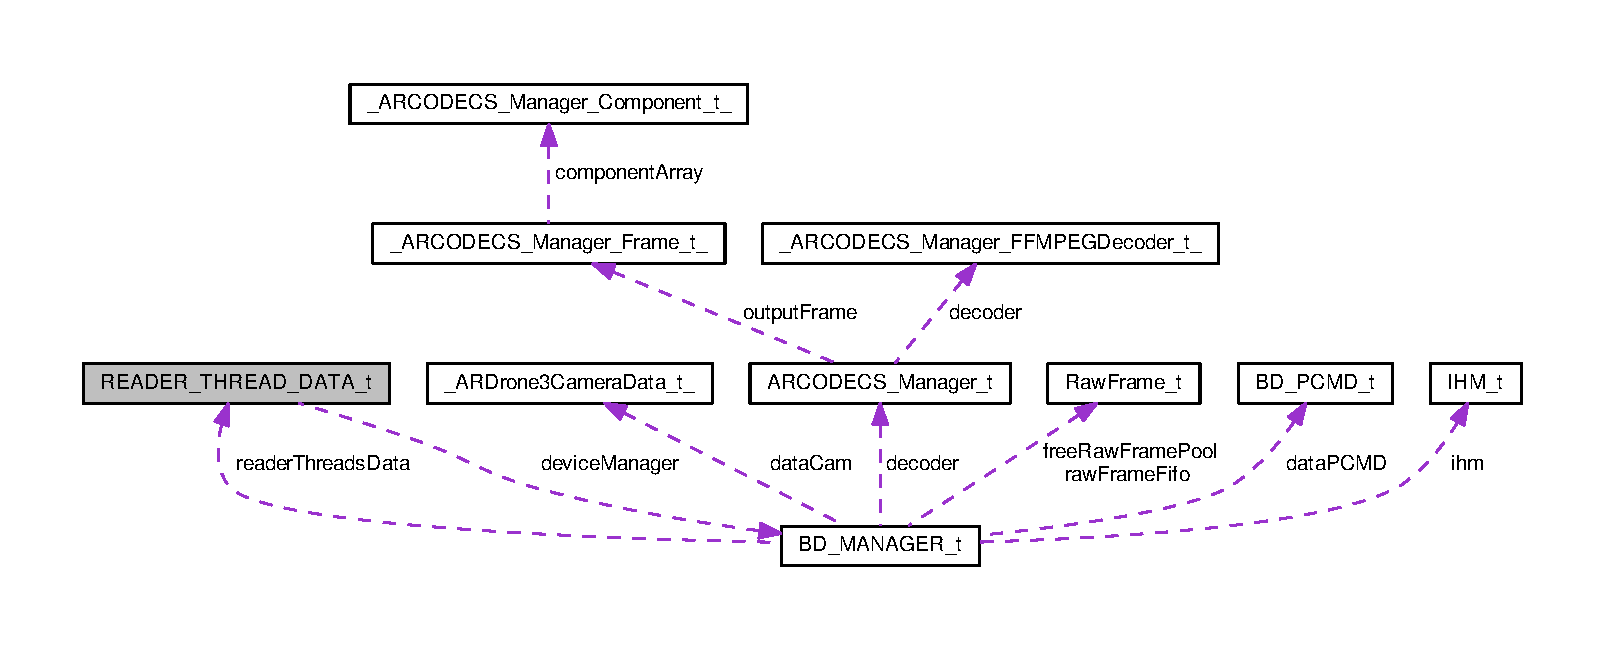
\includegraphics[width=350pt]{structREADER__THREAD__DATA__t__coll__graph}
\end{center}
\end{figure}
\subsection*{Public Attributes}
\begin{DoxyCompactItemize}
\item 
\hypertarget{structREADER__THREAD__DATA__t_a5b41dd4679caf26ca0d348df673cbab1}{}\hyperlink{structBD__MANAGER__t}{B\+D\+\_\+\+M\+A\+N\+A\+G\+E\+R\+\_\+t} $\ast$ {\bfseries device\+Manager}\label{structREADER__THREAD__DATA__t_a5b41dd4679caf26ca0d348df673cbab1}

\item 
\hypertarget{structREADER__THREAD__DATA__t_a58c42dc9083eb1a735d5c14fcbe4d75c}{}int {\bfseries reader\+Buffer\+Id}\label{structREADER__THREAD__DATA__t_a58c42dc9083eb1a735d5c14fcbe4d75c}

\end{DoxyCompactItemize}


The documentation for this struct was generated from the following file\+:\begin{DoxyCompactItemize}
\item 
Bebop\+Drone\+Decode\+Stream.\+h\end{DoxyCompactItemize}

\chapter{File Documentation}
\hypertarget{BebopDroneDecodeStream_8c}{}\section{Bebop\+Drone\+Decode\+Stream.\+c File Reference}
\label{BebopDroneDecodeStream_8c}\index{Bebop\+Drone\+Decode\+Stream.\+c@{Bebop\+Drone\+Decode\+Stream.\+c}}


This file contains sources about basic arsdk example decoding video stream from a Bebop\+Drone with ffmpeg.  


{\ttfamily \#include $<$stdlib.\+h$>$}\\*
{\ttfamily \#include $<$stdio.\+h$>$}\\*
{\ttfamily \#include $<$fcntl.\+h$>$}\\*
{\ttfamily \#include $<$string.\+h$>$}\\*
{\ttfamily \#include $<$unistd.\+h$>$}\\*
{\ttfamily \#include $<$signal.\+h$>$}\\*
{\ttfamily \#include $<$libavformat/avformat.\+h$>$}\\*
{\ttfamily \#include $<$libavcodec/avcodec.\+h$>$}\\*
{\ttfamily \#include $<$libavutil/imgutils.\+h$>$}\\*
{\ttfamily \#include $<$lib\+A\+R\+S\+A\+L/\+A\+R\+S\+A\+L.\+h$>$}\\*
{\ttfamily \#include $<$lib\+A\+R\+S\+A\+L/\+A\+R\+S\+A\+L\+\_\+\+Print.\+h$>$}\\*
{\ttfamily \#include $<$lib\+A\+R\+Network/\+A\+R\+Network.\+h$>$}\\*
{\ttfamily \#include $<$lib\+A\+R\+Network\+A\+L/\+A\+R\+Network\+A\+L.\+h$>$}\\*
{\ttfamily \#include $<$lib\+A\+R\+Discovery/\+A\+R\+Discovery.\+h$>$}\\*
{\ttfamily \#include $<$lib\+A\+R\+Stream/\+A\+R\+Stream.\+h$>$}\\*
{\ttfamily \#include \char`\"{}Bebop\+Drone\+Decode\+Stream.\+h\char`\"{}}\\*
Include dependency graph for Bebop\+Drone\+Decode\+Stream.\+c\+:
\nopagebreak
\begin{figure}[H]
\begin{center}
\leavevmode
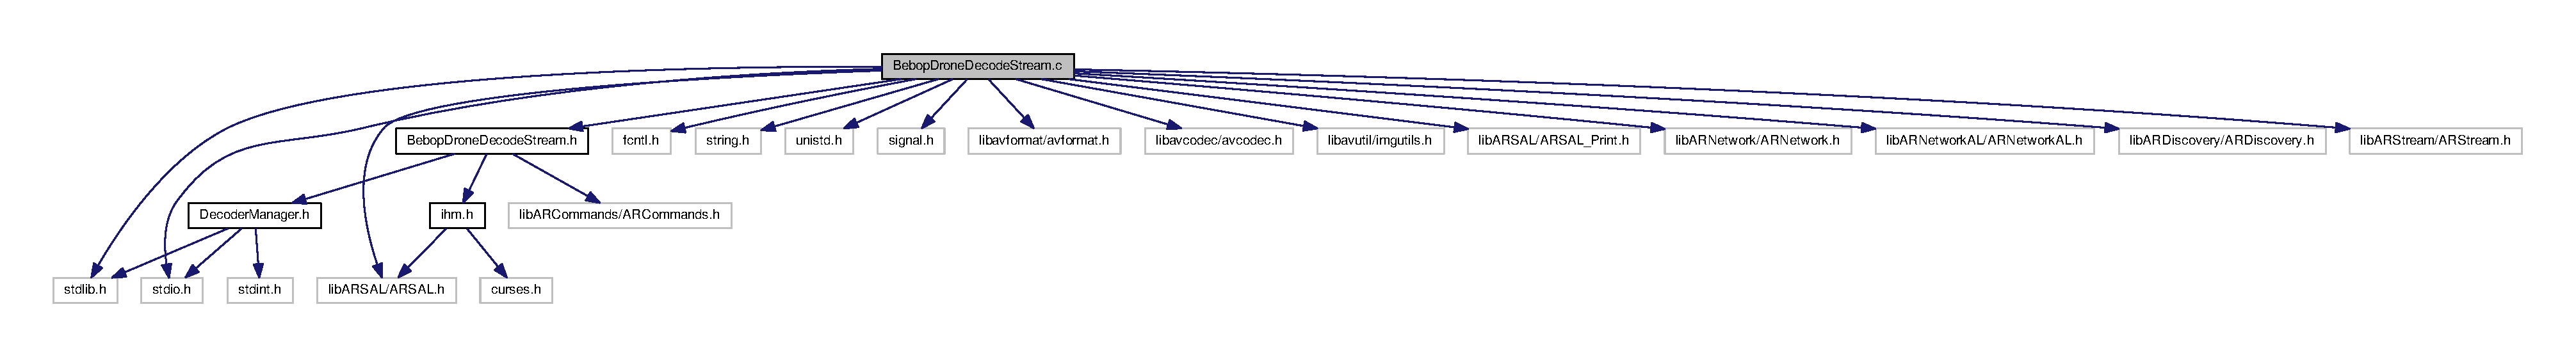
\includegraphics[width=350pt]{BebopDroneDecodeStream_8c__incl}
\end{center}
\end{figure}
\subsection*{Classes}
\begin{DoxyCompactItemize}
\item 
struct \hyperlink{structRawFrame__t}{Raw\+Frame\+\_\+t}
\begin{DoxyCompactList}\small\item\em Component of a frame. \end{DoxyCompactList}\end{DoxyCompactItemize}
\subsection*{Macros}
\begin{DoxyCompactItemize}
\item 
\hypertarget{BebopDroneDecodeStream_8c_afc3d101f633a076cc1ca84b85b6224b2}{}\#define {\bfseries T\+A\+G}~\char`\"{}Bebop\+Drone\+Receive\+Stream\char`\"{}\label{BebopDroneDecodeStream_8c_afc3d101f633a076cc1ca84b85b6224b2}

\item 
\hypertarget{BebopDroneDecodeStream_8c_adc013e0d9f61960f4fe071304a6c382e}{}\#define {\bfseries B\+D\+\_\+\+I\+P\+\_\+\+A\+D\+D\+R\+E\+S\+S}~\char`\"{}192.\+168.\+42.\+1\char`\"{}\label{BebopDroneDecodeStream_8c_adc013e0d9f61960f4fe071304a6c382e}

\item 
\hypertarget{BebopDroneDecodeStream_8c_a1c4908ea58b5fdf0a8ab4ab76b087363}{}\#define {\bfseries B\+D\+\_\+\+D\+I\+S\+C\+O\+V\+E\+R\+Y\+\_\+\+P\+O\+R\+T}~44444\label{BebopDroneDecodeStream_8c_a1c4908ea58b5fdf0a8ab4ab76b087363}

\item 
\hypertarget{BebopDroneDecodeStream_8c_a9a52aa0b24ad822bc2a71904fc13a4b0}{}\#define {\bfseries B\+D\+\_\+\+C2\+D\+\_\+\+P\+O\+R\+T}~54321\label{BebopDroneDecodeStream_8c_a9a52aa0b24ad822bc2a71904fc13a4b0}

\item 
\hypertarget{BebopDroneDecodeStream_8c_a7a8380e4998c7d3aa875daa140f91dc0}{}\#define {\bfseries B\+D\+\_\+\+D2\+C\+\_\+\+P\+O\+R\+T}~43210\label{BebopDroneDecodeStream_8c_a7a8380e4998c7d3aa875daa140f91dc0}

\item 
\hypertarget{BebopDroneDecodeStream_8c_aab580caea5e72eb22323754d9c8cc68f}{}\#define {\bfseries B\+D\+\_\+\+N\+E\+T\+\_\+\+C\+D\+\_\+\+N\+O\+N\+A\+C\+K\+\_\+\+I\+D}~10\label{BebopDroneDecodeStream_8c_aab580caea5e72eb22323754d9c8cc68f}

\item 
\hypertarget{BebopDroneDecodeStream_8c_a60fa904d11e4eaeecfd6f2508d013296}{}\#define {\bfseries B\+D\+\_\+\+N\+E\+T\+\_\+\+C\+D\+\_\+\+A\+C\+K\+\_\+\+I\+D}~11\label{BebopDroneDecodeStream_8c_a60fa904d11e4eaeecfd6f2508d013296}

\item 
\hypertarget{BebopDroneDecodeStream_8c_addd16331fccdec82496eb6d1494168f3}{}\#define {\bfseries B\+D\+\_\+\+N\+E\+T\+\_\+\+C\+D\+\_\+\+E\+M\+E\+R\+G\+E\+N\+C\+Y\+\_\+\+I\+D}~12\label{BebopDroneDecodeStream_8c_addd16331fccdec82496eb6d1494168f3}

\item 
\hypertarget{BebopDroneDecodeStream_8c_ac155a7aa415c6f19d9bc18eb5b3294fd}{}\#define {\bfseries B\+D\+\_\+\+N\+E\+T\+\_\+\+C\+D\+\_\+\+V\+I\+D\+E\+O\+\_\+\+A\+C\+K\+\_\+\+I\+D}~13\label{BebopDroneDecodeStream_8c_ac155a7aa415c6f19d9bc18eb5b3294fd}

\item 
\hypertarget{BebopDroneDecodeStream_8c_a33b2b60f79af99e36a36bd32ac19264f}{}\#define {\bfseries B\+D\+\_\+\+N\+E\+T\+\_\+\+D\+C\+\_\+\+N\+A\+V\+D\+A\+T\+A\+\_\+\+I\+D}~127\label{BebopDroneDecodeStream_8c_a33b2b60f79af99e36a36bd32ac19264f}

\item 
\hypertarget{BebopDroneDecodeStream_8c_aec4b42e6bc5ef48a8f46890fbb8ec774}{}\#define {\bfseries B\+D\+\_\+\+N\+E\+T\+\_\+\+D\+C\+\_\+\+E\+V\+E\+N\+T\+\_\+\+I\+D}~126\label{BebopDroneDecodeStream_8c_aec4b42e6bc5ef48a8f46890fbb8ec774}

\item 
\hypertarget{BebopDroneDecodeStream_8c_aa7c9d49af109dd610c0ad794fdca8a40}{}\#define {\bfseries B\+D\+\_\+\+N\+E\+T\+\_\+\+D\+C\+\_\+\+V\+I\+D\+E\+O\+\_\+\+D\+A\+T\+A\+\_\+\+I\+D}~125\label{BebopDroneDecodeStream_8c_aa7c9d49af109dd610c0ad794fdca8a40}

\item 
\hypertarget{BebopDroneDecodeStream_8c_a2b68f6f58d408d67633d2b2dbc500949}{}\#define {\bfseries B\+D\+\_\+\+N\+E\+T\+\_\+\+D\+C\+\_\+\+V\+I\+D\+E\+O\+\_\+\+F\+R\+A\+G\+\_\+\+S\+I\+Z\+E}~65000\label{BebopDroneDecodeStream_8c_a2b68f6f58d408d67633d2b2dbc500949}

\item 
\hypertarget{BebopDroneDecodeStream_8c_a9f457f37830d95376ab604ca8ab32f84}{}\#define {\bfseries B\+D\+\_\+\+N\+E\+T\+\_\+\+D\+C\+\_\+\+V\+I\+D\+E\+O\+\_\+\+M\+A\+X\+\_\+\+N\+U\+M\+B\+E\+R\+\_\+\+O\+F\+\_\+\+F\+R\+A\+G}~4\label{BebopDroneDecodeStream_8c_a9f457f37830d95376ab604ca8ab32f84}

\item 
\hypertarget{BebopDroneDecodeStream_8c_a441987ded0112a24887aa2c98aa73798}{}\#define {\bfseries B\+D\+\_\+\+R\+A\+W\+\_\+\+F\+R\+A\+M\+E\+\_\+\+B\+U\+F\+F\+E\+R\+\_\+\+S\+I\+Z\+E}~50\label{BebopDroneDecodeStream_8c_a441987ded0112a24887aa2c98aa73798}

\item 
\hypertarget{BebopDroneDecodeStream_8c_ad98c19cb9af7ea2507a1e6d39732ccfe}{}\#define {\bfseries B\+D\+\_\+\+R\+A\+W\+\_\+\+F\+R\+A\+M\+E\+\_\+\+P\+O\+O\+L\+\_\+\+S\+I\+Z\+E}~50\label{BebopDroneDecodeStream_8c_ad98c19cb9af7ea2507a1e6d39732ccfe}

\item 
\hypertarget{BebopDroneDecodeStream_8c_a2411ca45269a59691454ca7c3b0f34f5}{}\#define {\bfseries E\+R\+R\+O\+R\+\_\+\+S\+T\+R\+\_\+\+L\+E\+N\+G\+T\+H}~2048\label{BebopDroneDecodeStream_8c_a2411ca45269a59691454ca7c3b0f34f5}

\item 
\hypertarget{BebopDroneDecodeStream_8c_abc7fca69f0408724458bfe224397ad9c}{}\#define {\bfseries F\+I\+F\+O\+\_\+\+D\+I\+R\+\_\+\+P\+A\+T\+T\+E\+R\+N}~\char`\"{}/tmp/arsdk\+\_\+\+X\+X\+X\+X\+X\+X\char`\"{}\label{BebopDroneDecodeStream_8c_abc7fca69f0408724458bfe224397ad9c}

\item 
\hypertarget{BebopDroneDecodeStream_8c_a4e0d0f1b9bc23052255969da4c5ee560}{}\#define {\bfseries F\+I\+F\+O\+\_\+\+N\+A\+M\+E}~\char`\"{}arsdk\+\_\+fifo\char`\"{}\label{BebopDroneDecodeStream_8c_a4e0d0f1b9bc23052255969da4c5ee560}

\end{DoxyCompactItemize}
\subsection*{Functions}
\begin{DoxyCompactItemize}
\item 
int \hyperlink{BebopDroneDecodeStream_8c_a08bfd7b1c4195ed4b8b27bdf432f8ca2}{get\+Next\+Data\+Callback} (uint8\+\_\+t $\ast$$\ast$data, void $\ast$custom\+Data)
\item 
\hypertarget{BebopDroneDecodeStream_8c_a691cde673f17879b38d34df8275b21fe}{}void $\ast$ {\bfseries Decode\+\_\+\+Run\+Data\+Thread} (void $\ast$custom\+Data)\label{BebopDroneDecodeStream_8c_a691cde673f17879b38d34df8275b21fe}

\item 
\hypertarget{BebopDroneDecodeStream_8c_a4a44a241e01c20801739b64f9422068a}{}\hyperlink{structRawFrame__t}{Raw\+Frame\+\_\+t} $\ast$ {\bfseries get\+Free\+Raw\+Frame} (\hyperlink{structBD__MANAGER__t}{B\+D\+\_\+\+M\+A\+N\+A\+G\+E\+R\+\_\+t} $\ast$device\+Manager)\label{BebopDroneDecodeStream_8c_a4a44a241e01c20801739b64f9422068a}

\item 
\hypertarget{BebopDroneDecodeStream_8c_ab72dad3a5c7e1080803610a51530280c}{}void {\bfseries add\+Free\+Raw\+Frame\+To\+Fifo} (\hyperlink{structBD__MANAGER__t}{B\+D\+\_\+\+M\+A\+N\+A\+G\+E\+R\+\_\+t} $\ast$device\+Manager, \hyperlink{structRawFrame__t}{Raw\+Frame\+\_\+t} $\ast$raw\+Frame)\label{BebopDroneDecodeStream_8c_ab72dad3a5c7e1080803610a51530280c}

\item 
\hypertarget{BebopDroneDecodeStream_8c_a46c3c034ff0bfbedff5cdd6bc24f489e}{}void {\bfseries flush\+Fifo} (\hyperlink{structBD__MANAGER__t}{B\+D\+\_\+\+M\+A\+N\+A\+G\+E\+R\+\_\+t} $\ast$device\+Manager)\label{BebopDroneDecodeStream_8c_a46c3c034ff0bfbedff5cdd6bc24f489e}

\item 
\hypertarget{BebopDroneDecodeStream_8c_a2861f4ce82668c5a911c1f8f40d78ae5}{}void {\bfseries put\+Raw\+Frame\+Back\+To\+Pool} (\hyperlink{structBD__MANAGER__t}{B\+D\+\_\+\+M\+A\+N\+A\+G\+E\+R\+\_\+t} $\ast$device\+Manager, int fifo\+Idx)\label{BebopDroneDecodeStream_8c_a2861f4ce82668c5a911c1f8f40d78ae5}

\item 
\hypertarget{BebopDroneDecodeStream_8c_a8b2bb5235050c24fd99afd0433a776ee}{}\hyperlink{structRawFrame__t}{Raw\+Frame\+\_\+t} $\ast$ {\bfseries get\+Frame\+From\+Data} (\hyperlink{structBD__MANAGER__t}{B\+D\+\_\+\+M\+A\+N\+A\+G\+E\+R\+\_\+t} $\ast$device\+Manager, uint8\+\_\+t $\ast$data)\label{BebopDroneDecodeStream_8c_a8b2bb5235050c24fd99afd0433a776ee}

\item 
\hypertarget{BebopDroneDecodeStream_8c_a0ddf1224851353fc92bfbff6f499fa97}{}int {\bfseries main} (int argc, char $\ast$argv\mbox{[}$\,$\mbox{]})\label{BebopDroneDecodeStream_8c_a0ddf1224851353fc92bfbff6f499fa97}

\item 
int \hyperlink{BebopDroneDecodeStream_8c_a2b9b6a2446aa42bc9946d785335c04da}{ardiscovery\+Connect} (\hyperlink{structBD__MANAGER__t}{B\+D\+\_\+\+M\+A\+N\+A\+G\+E\+R\+\_\+t} $\ast$device\+Manager)
\item 
\hypertarget{BebopDroneDecodeStream_8c_a54ed290cab8b5d7753f8e1cfde7f3402}{}e\+A\+R\+D\+I\+S\+C\+O\+V\+E\+R\+Y\+\_\+\+E\+R\+R\+O\+R {\bfseries A\+R\+D\+I\+S\+C\+O\+V\+E\+R\+Y\+\_\+\+Connection\+\_\+\+Send\+Json\+Callback} (uint8\+\_\+t $\ast$data\+Tx, uint32\+\_\+t $\ast$data\+Tx\+Size, void $\ast$custom\+Data)\label{BebopDroneDecodeStream_8c_a54ed290cab8b5d7753f8e1cfde7f3402}

\item 
\hypertarget{BebopDroneDecodeStream_8c_af9c381937710e272ac4bd698f117eaf5}{}e\+A\+R\+D\+I\+S\+C\+O\+V\+E\+R\+Y\+\_\+\+E\+R\+R\+O\+R {\bfseries A\+R\+D\+I\+S\+C\+O\+V\+E\+R\+Y\+\_\+\+Connection\+\_\+\+Receive\+Json\+Callback} (uint8\+\_\+t $\ast$data\+Rx, uint32\+\_\+t data\+Rx\+Size, char $\ast$ip, void $\ast$custom\+Data)\label{BebopDroneDecodeStream_8c_af9c381937710e272ac4bd698f117eaf5}

\item 
int \hyperlink{BebopDroneDecodeStream_8c_a0543f6e06eaff63f731949547f3a85d8}{start\+Network} (\hyperlink{structBD__MANAGER__t}{B\+D\+\_\+\+M\+A\+N\+A\+G\+E\+R\+\_\+t} $\ast$device\+Manager)
\item 
\hypertarget{BebopDroneDecodeStream_8c_a8a5e86faf411bff72335ff9cf3895bfb}{}void {\bfseries stop\+Network} (\hyperlink{structBD__MANAGER__t}{B\+D\+\_\+\+M\+A\+N\+A\+G\+E\+R\+\_\+t} $\ast$device\+Manager)\label{BebopDroneDecodeStream_8c_a8a5e86faf411bff72335ff9cf3895bfb}

\item 
\hypertarget{BebopDroneDecodeStream_8c_aa2f6a23b311128cdafc9ace4481fa3a6}{}void {\bfseries on\+Disconnect\+Network} (A\+R\+N\+E\+T\+W\+O\+R\+K\+\_\+\+Manager\+\_\+t $\ast$manager, A\+R\+N\+E\+T\+W\+O\+R\+K\+A\+L\+\_\+\+Manager\+\_\+t $\ast$al\+Manager, void $\ast$custom\+Data)\label{BebopDroneDecodeStream_8c_aa2f6a23b311128cdafc9ace4481fa3a6}

\item 
int \hyperlink{BebopDroneDecodeStream_8c_a6d9fe62983b7fe68d35e9b316d60384d}{start\+Video} (\hyperlink{structBD__MANAGER__t}{B\+D\+\_\+\+M\+A\+N\+A\+G\+E\+R\+\_\+t} $\ast$device\+Manager)
\item 
\hypertarget{BebopDroneDecodeStream_8c_a468ec653188df139f2456902cae9601f}{}void {\bfseries stop\+Video} (\hyperlink{structBD__MANAGER__t}{B\+D\+\_\+\+M\+A\+N\+A\+G\+E\+R\+\_\+t} $\ast$device\+Manager)\label{BebopDroneDecodeStream_8c_a468ec653188df139f2456902cae9601f}

\item 
\hypertarget{BebopDroneDecodeStream_8c_ae9fd8e64a2ae42500d8c75a08be101d1}{}uint8\+\_\+t $\ast$ {\bfseries frame\+Complete\+Callback} (e\+A\+R\+S\+T\+R\+E\+A\+M\+\_\+\+R\+E\+A\+D\+E\+R\+\_\+\+C\+A\+U\+S\+E cause, uint8\+\_\+t $\ast$frame, uint32\+\_\+t frame\+Size, int number\+Of\+Skipped\+Frames, int is\+Flush\+Frame, uint32\+\_\+t $\ast$new\+Buffer\+Capacity, void $\ast$custom)\label{BebopDroneDecodeStream_8c_ae9fd8e64a2ae42500d8c75a08be101d1}

\item 
\hypertarget{BebopDroneDecodeStream_8c_a98dc5db13136ab0c9ab1c08ed3870474}{}int {\bfseries send\+P\+C\+M\+D} (\hyperlink{structBD__MANAGER__t}{B\+D\+\_\+\+M\+A\+N\+A\+G\+E\+R\+\_\+t} $\ast$device\+Manager)\label{BebopDroneDecodeStream_8c_a98dc5db13136ab0c9ab1c08ed3870474}

\item 
\hypertarget{BebopDroneDecodeStream_8c_aaf88d27f65c006348078b8ca94476410}{}int {\bfseries send\+Camera\+Orientation} (\hyperlink{structBD__MANAGER__t}{B\+D\+\_\+\+M\+A\+N\+A\+G\+E\+R\+\_\+t} $\ast$device\+Manager)\label{BebopDroneDecodeStream_8c_aaf88d27f65c006348078b8ca94476410}

\item 
\hypertarget{BebopDroneDecodeStream_8c_a26cd400731ae5cb29becf45c5f525ae7}{}int {\bfseries send\+Date} (\hyperlink{structBD__MANAGER__t}{B\+D\+\_\+\+M\+A\+N\+A\+G\+E\+R\+\_\+t} $\ast$device\+Manager)\label{BebopDroneDecodeStream_8c_a26cd400731ae5cb29becf45c5f525ae7}

\item 
\hypertarget{BebopDroneDecodeStream_8c_a7bb16065e10c67f43b404ddcdaf99d73}{}int {\bfseries send\+All\+Settings} (\hyperlink{structBD__MANAGER__t}{B\+D\+\_\+\+M\+A\+N\+A\+G\+E\+R\+\_\+t} $\ast$device\+Manager)\label{BebopDroneDecodeStream_8c_a7bb16065e10c67f43b404ddcdaf99d73}

\item 
\hypertarget{BebopDroneDecodeStream_8c_a49c2299419ff815bd57b393a03d5d5e3}{}int {\bfseries send\+All\+States} (\hyperlink{structBD__MANAGER__t}{B\+D\+\_\+\+M\+A\+N\+A\+G\+E\+R\+\_\+t} $\ast$device\+Manager)\label{BebopDroneDecodeStream_8c_a49c2299419ff815bd57b393a03d5d5e3}

\item 
\hypertarget{BebopDroneDecodeStream_8c_a887c5a9c4c6bfb020bb76959c9330efb}{}int {\bfseries send\+Begin\+Stream} (\hyperlink{structBD__MANAGER__t}{B\+D\+\_\+\+M\+A\+N\+A\+G\+E\+R\+\_\+t} $\ast$device\+Manager)\label{BebopDroneDecodeStream_8c_a887c5a9c4c6bfb020bb76959c9330efb}

\item 
\hypertarget{BebopDroneDecodeStream_8c_aa5132b6a63b4aea7d98ea6a92bfb9e5e}{}int {\bfseries send\+Takeoff} (\hyperlink{structBD__MANAGER__t}{B\+D\+\_\+\+M\+A\+N\+A\+G\+E\+R\+\_\+t} $\ast$device\+Manager)\label{BebopDroneDecodeStream_8c_aa5132b6a63b4aea7d98ea6a92bfb9e5e}

\item 
\hypertarget{BebopDroneDecodeStream_8c_a7d65b4f119d3cb15e2c3abd4fdc30f6d}{}int {\bfseries send\+Landing} (\hyperlink{structBD__MANAGER__t}{B\+D\+\_\+\+M\+A\+N\+A\+G\+E\+R\+\_\+t} $\ast$device\+Manager)\label{BebopDroneDecodeStream_8c_a7d65b4f119d3cb15e2c3abd4fdc30f6d}

\item 
\hypertarget{BebopDroneDecodeStream_8c_acad5459b948d07f347a90db9712d3304}{}int {\bfseries send\+Emergency} (\hyperlink{structBD__MANAGER__t}{B\+D\+\_\+\+M\+A\+N\+A\+G\+E\+R\+\_\+t} $\ast$device\+Manager)\label{BebopDroneDecodeStream_8c_acad5459b948d07f347a90db9712d3304}

\item 
e\+A\+R\+N\+E\+T\+W\+O\+R\+K\+\_\+\+M\+A\+N\+A\+G\+E\+R\+\_\+\+C\+A\+L\+L\+B\+A\+C\+K\+\_\+\+R\+E\+T\+U\+R\+N \hyperlink{BebopDroneDecodeStream_8c_a728f807e66dc811fa6772fb1340e6e92}{arnetwork\+Cmd\+Callback} (int buffer\+\_\+id, uint8\+\_\+t $\ast$data, void $\ast$custom, e\+A\+R\+N\+E\+T\+W\+O\+R\+K\+\_\+\+M\+A\+N\+A\+G\+E\+R\+\_\+\+C\+A\+L\+L\+B\+A\+C\+K\+\_\+\+S\+T\+A\+T\+U\+S cause)
\item 
void \hyperlink{BebopDroneDecodeStream_8c_aec865cd29eaaa088c75d7b4d97726201}{register\+A\+R\+Commands\+Callbacks} (\hyperlink{structBD__MANAGER__t}{B\+D\+\_\+\+M\+A\+N\+A\+G\+E\+R\+\_\+t} $\ast$device\+Manager)
\item 
\hypertarget{BebopDroneDecodeStream_8c_a334544c60e7a7f8d430b95d75c2dbc4b}{}void {\bfseries unregister\+A\+R\+Commands\+Callbacks} (void)\label{BebopDroneDecodeStream_8c_a334544c60e7a7f8d430b95d75c2dbc4b}

\item 
\hypertarget{BebopDroneDecodeStream_8c_a2e1acc68151890254450a1489e4c699b}{}void {\bfseries battery\+State\+Changed\+Callback} (uint8\+\_\+t percent, void $\ast$custom)\label{BebopDroneDecodeStream_8c_a2e1acc68151890254450a1489e4c699b}

\item 
\hypertarget{BebopDroneDecodeStream_8c_a5fca32daf44f156544e8682b5b59dccb}{}void {\bfseries flying\+State\+Changed\+Callback} (e\+A\+R\+C\+O\+M\+M\+A\+N\+D\+S\+\_\+\+A\+R\+D\+R\+O\+N\+E3\+\_\+\+P\+I\+L\+O\+T\+I\+N\+G\+S\+T\+A\+T\+E\+\_\+\+F\+L\+Y\+I\+N\+G\+S\+T\+A\+T\+E\+C\+H\+A\+N\+G\+E\+D\+\_\+\+S\+T\+A\+T\+E state, void $\ast$custom)\label{BebopDroneDecodeStream_8c_a5fca32daf44f156544e8682b5b59dccb}

\item 
int \hyperlink{BebopDroneDecodeStream_8c_a02995257f549a6f2978a01d670156848}{start\+Decoder} (\hyperlink{structBD__MANAGER__t}{B\+D\+\_\+\+M\+A\+N\+A\+G\+E\+R\+\_\+t} $\ast$device\+Manager)
\item 
\hypertarget{BebopDroneDecodeStream_8c_a1b2156ee0ef231027011827dbd7b090b}{}void {\bfseries stop\+Decoder} (\hyperlink{structBD__MANAGER__t}{B\+D\+\_\+\+M\+A\+N\+A\+G\+E\+R\+\_\+t} $\ast$device\+Manager)\label{BebopDroneDecodeStream_8c_a1b2156ee0ef231027011827dbd7b090b}

\item 
void \hyperlink{BebopDroneDecodeStream_8c_a3bcbfca6eea9b5388a9ccbe000598e71}{on\+Input\+Event} (e\+I\+H\+M\+\_\+\+I\+N\+P\+U\+T\+\_\+\+E\+V\+E\+N\+T event, void $\ast$custom\+Data)
\item 
\hypertarget{BebopDroneDecodeStream_8c_aaebc87fd1d07a699d3b9f1ebd0791896}{}int {\bfseries custom\+Print\+Callback} (e\+A\+R\+S\+A\+L\+\_\+\+P\+R\+I\+N\+T\+\_\+\+L\+E\+V\+E\+L level, const char $\ast$tag, const char $\ast$format, va\+\_\+list va)\label{BebopDroneDecodeStream_8c_aaebc87fd1d07a699d3b9f1ebd0791896}

\end{DoxyCompactItemize}
\subsection*{Variables}
\begin{DoxyCompactItemize}
\item 
\hypertarget{BebopDroneDecodeStream_8c_a7d2ca1ba0336e57f2500231a6ca05091}{}int {\bfseries g\+I\+H\+M\+Run} = 0\label{BebopDroneDecodeStream_8c_a7d2ca1ba0336e57f2500231a6ca05091}

\item 
\hypertarget{BebopDroneDecodeStream_8c_a1f61d9e9cc96aa362c377e65aa9e408e}{}char {\bfseries g\+Error\+Str} \mbox{[}E\+R\+R\+O\+R\+\_\+\+S\+T\+R\+\_\+\+L\+E\+N\+G\+T\+H\mbox{]}\label{BebopDroneDecodeStream_8c_a1f61d9e9cc96aa362c377e65aa9e408e}

\end{DoxyCompactItemize}


\subsection{Detailed Description}
This file contains sources about basic arsdk example decoding video stream from a Bebop\+Drone with ffmpeg. 

\begin{DoxyDate}{Date}
08/01/2015 
\end{DoxyDate}


\subsection{Function Documentation}
\hypertarget{BebopDroneDecodeStream_8c_a2b9b6a2446aa42bc9946d785335c04da}{}\index{Bebop\+Drone\+Decode\+Stream.\+c@{Bebop\+Drone\+Decode\+Stream.\+c}!ardiscovery\+Connect@{ardiscovery\+Connect}}
\index{ardiscovery\+Connect@{ardiscovery\+Connect}!Bebop\+Drone\+Decode\+Stream.\+c@{Bebop\+Drone\+Decode\+Stream.\+c}}
\subsubsection[{ardiscovery\+Connect}]{\setlength{\rightskip}{0pt plus 5cm}int ardiscovery\+Connect (
\begin{DoxyParamCaption}
\item[{{\bf B\+D\+\_\+\+M\+A\+N\+A\+G\+E\+R\+\_\+t} $\ast$}]{device\+Manager}
\end{DoxyParamCaption}
)}\label{BebopDroneDecodeStream_8c_a2b9b6a2446aa42bc9946d785335c04da}
Connection part \hypertarget{BebopDroneDecodeStream_8c_a728f807e66dc811fa6772fb1340e6e92}{}\index{Bebop\+Drone\+Decode\+Stream.\+c@{Bebop\+Drone\+Decode\+Stream.\+c}!arnetwork\+Cmd\+Callback@{arnetwork\+Cmd\+Callback}}
\index{arnetwork\+Cmd\+Callback@{arnetwork\+Cmd\+Callback}!Bebop\+Drone\+Decode\+Stream.\+c@{Bebop\+Drone\+Decode\+Stream.\+c}}
\subsubsection[{arnetwork\+Cmd\+Callback}]{\setlength{\rightskip}{0pt plus 5cm}e\+A\+R\+N\+E\+T\+W\+O\+R\+K\+\_\+\+M\+A\+N\+A\+G\+E\+R\+\_\+\+C\+A\+L\+L\+B\+A\+C\+K\+\_\+\+R\+E\+T\+U\+R\+N arnetwork\+Cmd\+Callback (
\begin{DoxyParamCaption}
\item[{int}]{buffer\+\_\+id, }
\item[{uint8\+\_\+t $\ast$}]{data, }
\item[{void $\ast$}]{custom, }
\item[{e\+A\+R\+N\+E\+T\+W\+O\+R\+K\+\_\+\+M\+A\+N\+A\+G\+E\+R\+\_\+\+C\+A\+L\+L\+B\+A\+C\+K\+\_\+\+S\+T\+A\+T\+U\+S}]{cause}
\end{DoxyParamCaption}
)}\label{BebopDroneDecodeStream_8c_a728f807e66dc811fa6772fb1340e6e92}
Commands part \hypertarget{BebopDroneDecodeStream_8c_a08bfd7b1c4195ed4b8b27bdf432f8ca2}{}\index{Bebop\+Drone\+Decode\+Stream.\+c@{Bebop\+Drone\+Decode\+Stream.\+c}!get\+Next\+Data\+Callback@{get\+Next\+Data\+Callback}}
\index{get\+Next\+Data\+Callback@{get\+Next\+Data\+Callback}!Bebop\+Drone\+Decode\+Stream.\+c@{Bebop\+Drone\+Decode\+Stream.\+c}}
\subsubsection[{get\+Next\+Data\+Callback}]{\setlength{\rightskip}{0pt plus 5cm}int get\+Next\+Data\+Callback (
\begin{DoxyParamCaption}
\item[{uint8\+\_\+t $\ast$$\ast$}]{data, }
\item[{void $\ast$}]{custom\+Data}
\end{DoxyParamCaption}
)}\label{BebopDroneDecodeStream_8c_a08bfd7b1c4195ed4b8b27bdf432f8ca2}
Handle older ffmpeg/libav versions \hypertarget{BebopDroneDecodeStream_8c_a3bcbfca6eea9b5388a9ccbe000598e71}{}\index{Bebop\+Drone\+Decode\+Stream.\+c@{Bebop\+Drone\+Decode\+Stream.\+c}!on\+Input\+Event@{on\+Input\+Event}}
\index{on\+Input\+Event@{on\+Input\+Event}!Bebop\+Drone\+Decode\+Stream.\+c@{Bebop\+Drone\+Decode\+Stream.\+c}}
\subsubsection[{on\+Input\+Event}]{\setlength{\rightskip}{0pt plus 5cm}void on\+Input\+Event (
\begin{DoxyParamCaption}
\item[{e\+I\+H\+M\+\_\+\+I\+N\+P\+U\+T\+\_\+\+E\+V\+E\+N\+T}]{event, }
\item[{void $\ast$}]{custom\+Data}
\end{DoxyParamCaption}
)}\label{BebopDroneDecodeStream_8c_a3bcbfca6eea9b5388a9ccbe000598e71}
I\+H\+M callbacks \hypertarget{BebopDroneDecodeStream_8c_aec865cd29eaaa088c75d7b4d97726201}{}\index{Bebop\+Drone\+Decode\+Stream.\+c@{Bebop\+Drone\+Decode\+Stream.\+c}!register\+A\+R\+Commands\+Callbacks@{register\+A\+R\+Commands\+Callbacks}}
\index{register\+A\+R\+Commands\+Callbacks@{register\+A\+R\+Commands\+Callbacks}!Bebop\+Drone\+Decode\+Stream.\+c@{Bebop\+Drone\+Decode\+Stream.\+c}}
\subsubsection[{register\+A\+R\+Commands\+Callbacks}]{\setlength{\rightskip}{0pt plus 5cm}void register\+A\+R\+Commands\+Callbacks (
\begin{DoxyParamCaption}
\item[{{\bf B\+D\+\_\+\+M\+A\+N\+A\+G\+E\+R\+\_\+t} $\ast$}]{device\+Manager}
\end{DoxyParamCaption}
)}\label{BebopDroneDecodeStream_8c_aec865cd29eaaa088c75d7b4d97726201}
Commands callback part \hypertarget{BebopDroneDecodeStream_8c_a02995257f549a6f2978a01d670156848}{}\index{Bebop\+Drone\+Decode\+Stream.\+c@{Bebop\+Drone\+Decode\+Stream.\+c}!start\+Decoder@{start\+Decoder}}
\index{start\+Decoder@{start\+Decoder}!Bebop\+Drone\+Decode\+Stream.\+c@{Bebop\+Drone\+Decode\+Stream.\+c}}
\subsubsection[{start\+Decoder}]{\setlength{\rightskip}{0pt plus 5cm}int start\+Decoder (
\begin{DoxyParamCaption}
\item[{{\bf B\+D\+\_\+\+M\+A\+N\+A\+G\+E\+R\+\_\+t} $\ast$}]{device\+Manager}
\end{DoxyParamCaption}
)}\label{BebopDroneDecodeStream_8c_a02995257f549a6f2978a01d670156848}
decoding part \hypertarget{BebopDroneDecodeStream_8c_a0543f6e06eaff63f731949547f3a85d8}{}\index{Bebop\+Drone\+Decode\+Stream.\+c@{Bebop\+Drone\+Decode\+Stream.\+c}!start\+Network@{start\+Network}}
\index{start\+Network@{start\+Network}!Bebop\+Drone\+Decode\+Stream.\+c@{Bebop\+Drone\+Decode\+Stream.\+c}}
\subsubsection[{start\+Network}]{\setlength{\rightskip}{0pt plus 5cm}int start\+Network (
\begin{DoxyParamCaption}
\item[{{\bf B\+D\+\_\+\+M\+A\+N\+A\+G\+E\+R\+\_\+t} $\ast$}]{device\+Manager}
\end{DoxyParamCaption}
)}\label{BebopDroneDecodeStream_8c_a0543f6e06eaff63f731949547f3a85d8}
Network part \hypertarget{BebopDroneDecodeStream_8c_a6d9fe62983b7fe68d35e9b316d60384d}{}\index{Bebop\+Drone\+Decode\+Stream.\+c@{Bebop\+Drone\+Decode\+Stream.\+c}!start\+Video@{start\+Video}}
\index{start\+Video@{start\+Video}!Bebop\+Drone\+Decode\+Stream.\+c@{Bebop\+Drone\+Decode\+Stream.\+c}}
\subsubsection[{start\+Video}]{\setlength{\rightskip}{0pt plus 5cm}int start\+Video (
\begin{DoxyParamCaption}
\item[{{\bf B\+D\+\_\+\+M\+A\+N\+A\+G\+E\+R\+\_\+t} $\ast$}]{device\+Manager}
\end{DoxyParamCaption}
)}\label{BebopDroneDecodeStream_8c_a6d9fe62983b7fe68d35e9b316d60384d}
Video part 
\hypertarget{ihm_8c}{}\section{ihm.\+c File Reference}
\label{ihm_8c}\index{ihm.\+c@{ihm.\+c}}


This file contains sources about ncurses I\+H\+M used by arsdk example \char`\"{}\+Bebop\+Drone\+Decode\+Stream\char`\"{}.  


{\ttfamily \#include $<$stdlib.\+h$>$}\\*
{\ttfamily \#include $<$curses.\+h$>$}\\*
{\ttfamily \#include $<$string.\+h$>$}\\*
{\ttfamily \#include $<$lib\+A\+R\+S\+A\+L/\+A\+R\+S\+A\+L.\+h$>$}\\*
{\ttfamily \#include \char`\"{}ihm.\+h\char`\"{}}\\*
Include dependency graph for ihm.\+c\+:
\nopagebreak
\begin{figure}[H]
\begin{center}
\leavevmode
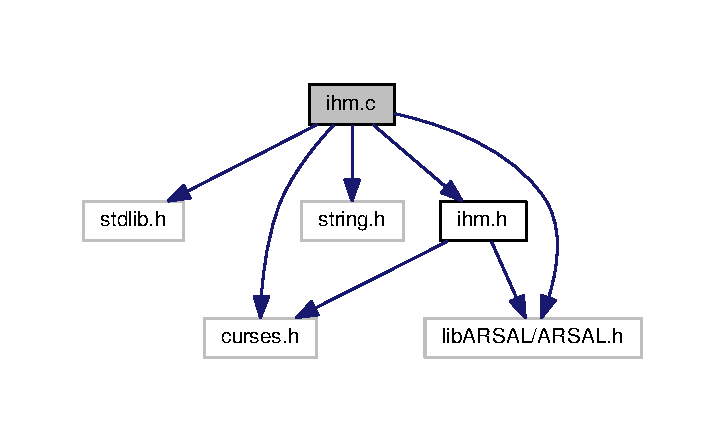
\includegraphics[width=348pt]{ihm_8c__incl}
\end{center}
\end{figure}
\subsection*{Macros}
\begin{DoxyCompactItemize}
\item 
\hypertarget{ihm_8c_a58017ec045269446009126ad5f844356}{}\#define {\bfseries H\+E\+A\+D\+E\+R\+\_\+\+X}~0\label{ihm_8c_a58017ec045269446009126ad5f844356}

\item 
\hypertarget{ihm_8c_add11cdd656672eaeef4410dda5937b0d}{}\#define {\bfseries H\+E\+A\+D\+E\+R\+\_\+\+Y}~0\label{ihm_8c_add11cdd656672eaeef4410dda5937b0d}

\item 
\hypertarget{ihm_8c_abe06bdb66452ea025f4ca3117856e54c}{}\#define {\bfseries I\+N\+S\+T\+R\+U\+C\+T\+I\+O\+N\+\_\+\+X}~0\label{ihm_8c_abe06bdb66452ea025f4ca3117856e54c}

\item 
\hypertarget{ihm_8c_a0661a392db40be1552f576a54f1c8c33}{}\#define {\bfseries I\+N\+S\+T\+R\+U\+C\+T\+I\+O\+N\+\_\+\+Y}~2\label{ihm_8c_a0661a392db40be1552f576a54f1c8c33}

\item 
\hypertarget{ihm_8c_a23cab0b49444cc4870f0d671f3d03ace}{}\#define {\bfseries B\+A\+T\+T\+E\+R\+Y\+\_\+\+X}~0\label{ihm_8c_a23cab0b49444cc4870f0d671f3d03ace}

\item 
\hypertarget{ihm_8c_a94ccb05dea98d7f090d5af6a7143eacb}{}\#define {\bfseries B\+A\+T\+T\+E\+R\+Y\+\_\+\+Y}~10\label{ihm_8c_a94ccb05dea98d7f090d5af6a7143eacb}

\item 
\hypertarget{ihm_8c_a741dafa1bd1ea79378f402bb15fbeeca}{}\#define {\bfseries I\+N\+F\+O\+\_\+\+X}~0\label{ihm_8c_a741dafa1bd1ea79378f402bb15fbeeca}

\item 
\hypertarget{ihm_8c_a89904cb639d01dbee42b37befc20650c}{}\#define {\bfseries I\+N\+F\+O\+\_\+\+Y}~12\label{ihm_8c_a89904cb639d01dbee42b37befc20650c}

\end{DoxyCompactItemize}
\subsection*{Functions}
\begin{DoxyCompactItemize}
\item 
\hypertarget{ihm_8c_a745d6e022c26b5c342d0c452be45daba}{}void $\ast$ {\bfseries I\+H\+M\+\_\+\+Input\+Processing} (void $\ast$data)\label{ihm_8c_a745d6e022c26b5c342d0c452be45daba}

\item 
\hypertarget{ihm_8c_a0c80596eb686749500f4f028f1b96e03}{}\hyperlink{structIHM__t}{I\+H\+M\+\_\+t} $\ast$ {\bfseries I\+H\+M\+\_\+\+New} (I\+H\+M\+\_\+on\+Input\+Event\+\_\+t on\+Input\+Event\+Callback)\label{ihm_8c_a0c80596eb686749500f4f028f1b96e03}

\item 
\hypertarget{ihm_8c_a16fdfbb07176c17e294bbd2aff53f36d}{}void {\bfseries I\+H\+M\+\_\+\+Delete} (\hyperlink{structIHM__t}{I\+H\+M\+\_\+t} $\ast$$\ast$ihm)\label{ihm_8c_a16fdfbb07176c17e294bbd2aff53f36d}

\item 
\hypertarget{ihm_8c_ae15b885587a1ad3ce40cd267a15d4ab9}{}void {\bfseries I\+H\+M\+\_\+set\+Custom\+Data} (\hyperlink{structIHM__t}{I\+H\+M\+\_\+t} $\ast$ihm, void $\ast$custom\+Data)\label{ihm_8c_ae15b885587a1ad3ce40cd267a15d4ab9}

\item 
\hypertarget{ihm_8c_a026e2b72ec609344806c307c4946fd07}{}void {\bfseries I\+H\+M\+\_\+\+Print\+Header} (\hyperlink{structIHM__t}{I\+H\+M\+\_\+t} $\ast$ihm, char $\ast$header\+Str)\label{ihm_8c_a026e2b72ec609344806c307c4946fd07}

\item 
\hypertarget{ihm_8c_a1b4881214982f377f9d7edcef574ff5f}{}void {\bfseries I\+H\+M\+\_\+\+Print\+Instruction} (\hyperlink{structIHM__t}{I\+H\+M\+\_\+t} $\ast$ihm, char $\ast$instruction\+Str)\label{ihm_8c_a1b4881214982f377f9d7edcef574ff5f}

\item 
\hypertarget{ihm_8c_ae9098136f2de628d2537fd84eba10b1e}{}void {\bfseries I\+H\+M\+\_\+\+Print\+Info} (\hyperlink{structIHM__t}{I\+H\+M\+\_\+t} $\ast$ihm, char $\ast$info\+Str)\label{ihm_8c_ae9098136f2de628d2537fd84eba10b1e}

\item 
\hypertarget{ihm_8c_af0d8adaf58223e18f35ea379ebeb5dbd}{}void {\bfseries I\+H\+M\+\_\+\+Print\+Battery} (\hyperlink{structIHM__t}{I\+H\+M\+\_\+t} $\ast$ihm, uint8\+\_\+t percent)\label{ihm_8c_af0d8adaf58223e18f35ea379ebeb5dbd}

\end{DoxyCompactItemize}


\subsection{Detailed Description}
This file contains sources about ncurses I\+H\+M used by arsdk example \char`\"{}\+Bebop\+Drone\+Decode\+Stream\char`\"{}. 

\begin{DoxyDate}{Date}
15/01/2015 
\end{DoxyDate}

%--- End generated contents ---

% Index
\backmatter
\newpage
\phantomsection
\clearemptydoublepage
\addcontentsline{toc}{chapter}{Index}
\printindex

\end{document}
